% =============================================================================
% O PROBLEMA DO CONTRAFACTUAL (14:20 a 14:30)   [Script 01]
% =============================================================================
\section[Contrafactual]{O problema do contrafactual}
\subsection{O problema}

\begin{frame}{O problema fundamental da inferência causal}
  Para cada pessoa só observamos \destaque{um} dos dois mundos:
  \vspace{0.2cm}
  \begin{center}
  \footnotesize
  \renewcommand{\arraystretch}{1.25}
  \begin{tabular}{lcccc}
    \toprule
    & \textbf{Participou?} & \textbf{Com programa} & \textbf{Sem programa} & \textbf{Efeito} \\ \midrule
    Ana   & sim & R\$ 2.400 & \destaque{?} & \destaque{?} \\
    Bruno & não & \destaque{?} & R\$ 2.000 & \destaque{?} \\
    Carla & sim & R\$ 2.700 & \destaque{?} & \destaque{?} \\
    Davi  & não & \destaque{?} & R\$ 1.800 & \destaque{?} \\ \bottomrule
  \end{tabular}
  \end{center}
  \vspace{0.2cm}
  \small O que não observamos é o \ind{contrafactual}. Toda técnica de avaliação de impacto é uma \destaque{estratégia para estimá-lo}.
\end{frame}

\begin{frame}{O contrafactual: a comparação ideal}
  \centering
  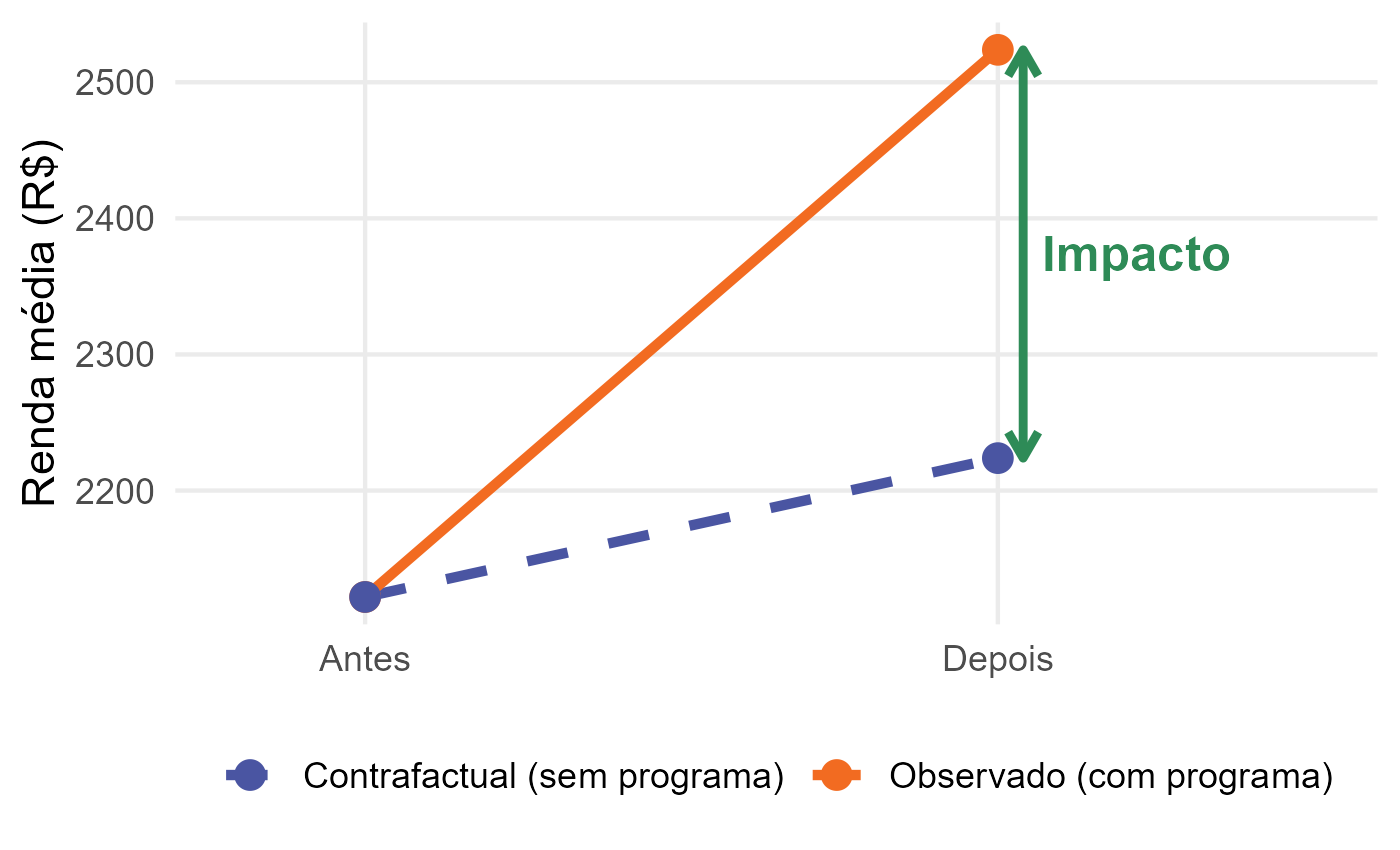
\includegraphics[height=4.6cm]{01_contrafactual.png}\par
  \footnotesize A linha tracejada nunca é observada na vida real. Só numa \ind{simulação} podemos desenhá-la.
\end{frame}

\begin{frame}{Dois falsos contrafactuais}
  \begin{columns}[T]
    \begin{column}{0.5\textwidth}
      \begin{block}{Participantes $\times$ não participantes}
        \footnotesize
        Quem participa é diferente de quem não participa (mais motivado, mais escolarizado).\\[3pt]
        \destaque{Viés de seleção.}
      \end{block}
    \end{column}
    \begin{column}{0.5\textwidth}
      \begin{block}{Antes $\times$ depois}
        \footnotesize
        A renda pode ter subido por crescimento econômico, inflação, ciclo de vida.\\[3pt]
        \destaque{Tendência no tempo.}
      \end{block}
    \end{column}
  \end{columns}
  \vspace{0.2cm}
  \centering\small Nos dois casos o efeito do programa se mistura com outros fatores.
  \vspace{0.1cm}
  \begin{block}{Voltando à enquete (dados simulados do \textit{Qualifica}, efeito verdadeiro R\$ 300)}
    \footnotesize Participantes $\times$ não: R\$ 587 (\destaque{+287}, seleção). Antes $\times$ depois: R\$ 402 (\destaque{+102}, tendência). Resposta (b): o efeito é \textbf{menor}.
  \end{block}
\end{frame}

\begin{frame}{Viés de seleção: os grupos já eram diferentes}
  \centering
  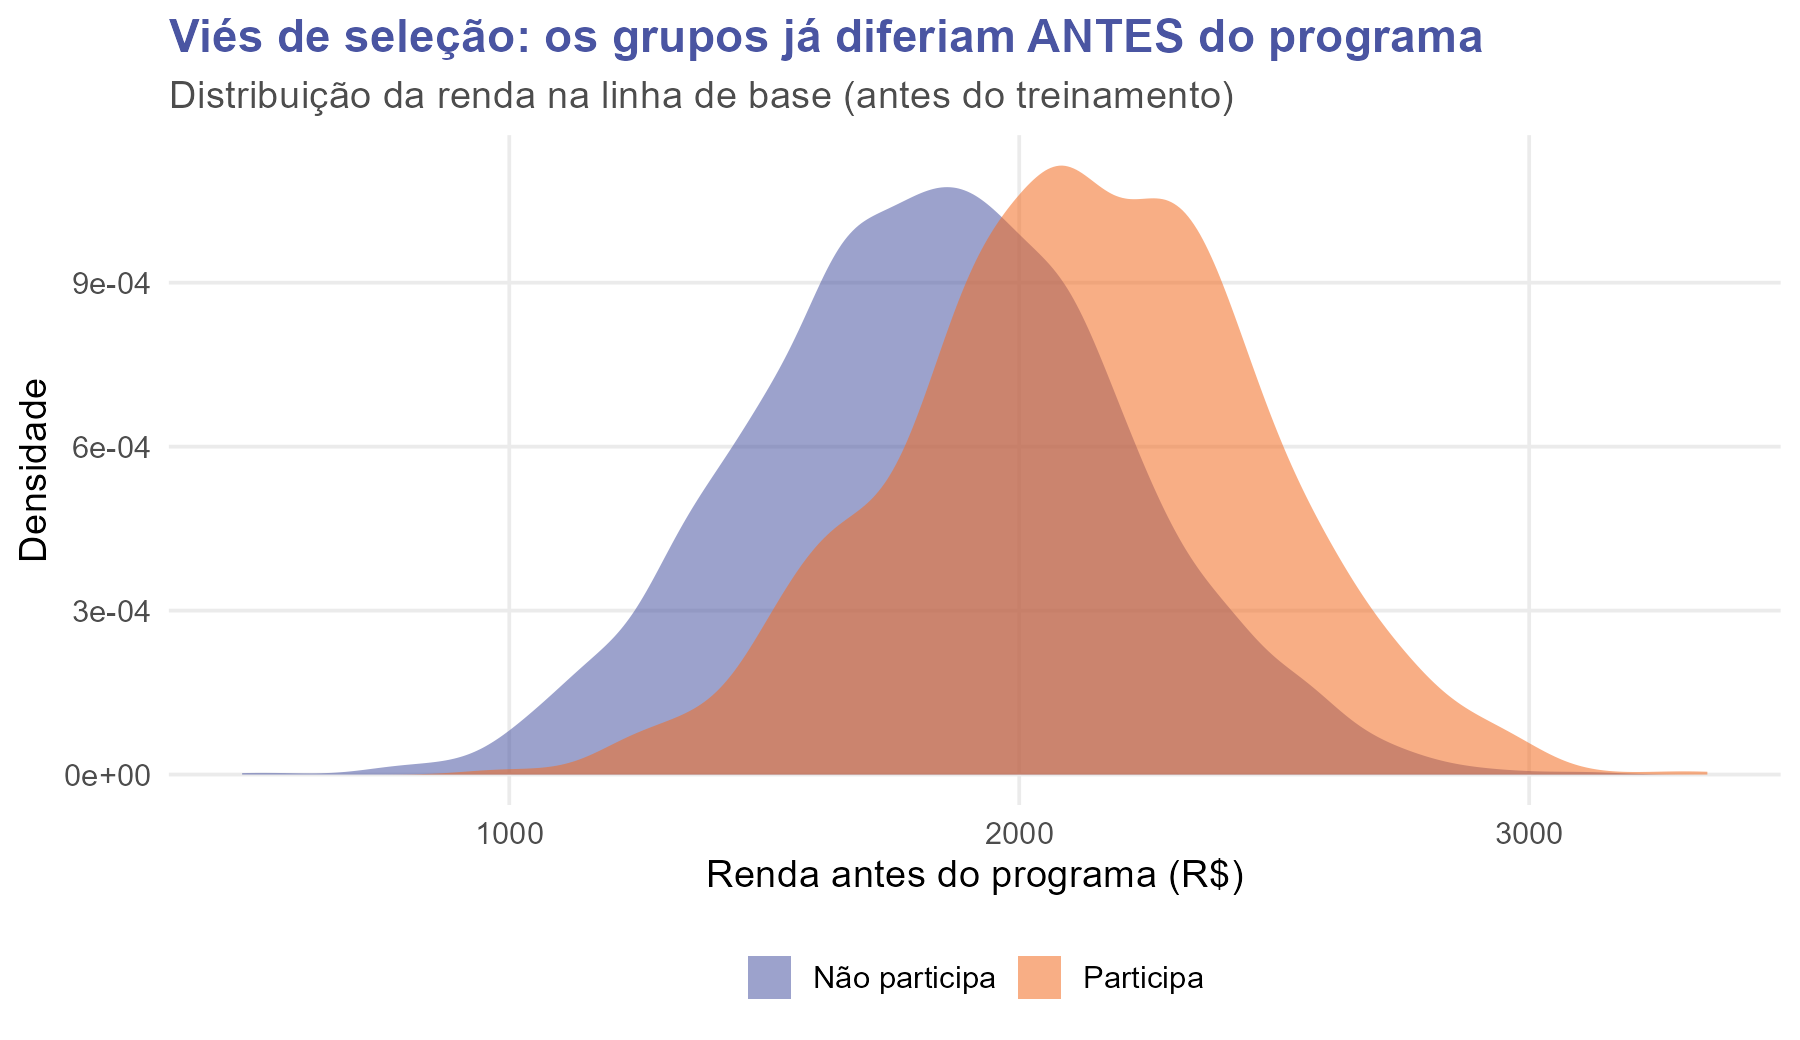
\includegraphics[height=4.2cm]{01_vies_selecao.png}\par
  \footnotesize Renda \textbf{antes} do programa: participantes R\$ 2.122; não participantes R\$ 1.836. A motivação (não observada) também difere.
\end{frame}

\subsection{Características}

\begin{frame}{Características de um bom contrafactual}
  \scriptsize
  \renewcommand{\arraystretch}{1.25}
  \begin{tabularx}{\textwidth}{@{}>{\bfseries\color{azul}\raggedright\arraybackslash}p{2.5cm}>{\raggedright\arraybackslash}X>{\raggedright\arraybackslash}X@{}}
    \toprule
    Característica & O que significa & Como checar \\ \midrule
    Comparável antes & Mesmo nível e trajetória antes da política & Balanço; pré-tendências \\
    Seleção independente & Quem entra não foi escolhido pelo que espera ganhar & Desenho (sorteio, regra) \\
    Mesmos choques & Os grupos enfrentam o mesmo contexto e período & Dados de antes e depois \\
    Sem contaminação & O controle não recebe efeitos indiretos & Distância entre unidades \\
    Mesma medida & Resultado medido igual, sem perda seletiva & Taxa de resposta por grupo \\ \bottomrule
  \end{tabularx}
  \vspace{0.2cm}\par
  \small Cada técnica garante essas características de um jeito: o \textbf{sorteio}, o \textbf{gêmeo}, a \textbf{tendência paralela}, o \textbf{corte}.
\end{frame}

\begin{frame}{Mapa das técnicas}
  \centering
  \begin{tikzpicture}[scale=0.8,every node/.style={transform shape}]
    \node[cxl,minimum width=4.2cm,minimum height=0.8cm,font=\small\bfseries] (top) at (0,0) {Identificar o impacto causal};
    \node[cxi,minimum width=3.4cm] (exp) at (-4.3,-1.7) {\textbf{Experimento}\\sorteio entre elegíveis\\(ou natural)};
    \node[cx,minimum width=3.6cm] (qe) at (1.8,-1.7) {\textbf{Quase-experimentos}\\(dados observacionais)};
    \draw[seta] (top) -- (exp); \draw[seta] (top) -- (qe);
    \node[cxi,minimum width=2.1cm] (psm) at (-1.6,-4.1) {\textbf{Pareamento}\\``gêmeos''\\observados};
    \node[cxi,minimum width=2.1cm] (did) at (1.0,-4.1) {\textbf{Dif.-em-dif.}\\tendência do\\controle};
    \node[cxi,minimum width=2.1cm] (rdd) at (3.6,-4.1) {\textbf{Reg. descont.}\\corte de\\elegibilidade};
    \node[cx,minimum width=2.1cm] (out) at (6.2,-4.1) {\textbf{Outras}\\IV, sintético,\\ponderação};
    \foreach \x in {psm,did,rdd,out} { \draw[seta] (qe) -- (\x); }
  \end{tikzpicture}
\end{frame}
